\section{Testing}
\subsection{Microservices}
\subsubsection{Tests of a single microservices}
For managing the tests, in general, during the development, once a feature was ready it was tested. 
The procedure described in the Design document was followed; however, due to the fact that many spring
components and classes do already many things, unit tests of single class sometimes didn't make much 
sense, because it would have been necessary to mock many Spring features, that are supposed to be already
tested and working properly. \\
For the projects, the process of testing usually followed this life cycle: repositories have been tested firsts, then the services, that cover
the business functions of the project under consideration, and then the controllers, for which two kinds of tests were performed: a unit and
an integration test.
These integration tests involves all the stacks that were developed in the projects: indeed, from here, the connection to the APIs with HTTP/
HTTPS requests are tested: this methods usually call the business functions, that modifies the databases by means of repositories.
If error occurs, the classes in the advice packages come into help, and, therefore, they are tested as well. \\
For what concerns the tests that regards interfaces that allows to share events with other microservices, as soon as it was possible to have
them working they were tested as well. 
However, it is worth to note that the real integration between microservices have been tested with JMeter. This is because there were multiple projects and an integration test with JUnit should have been done on one of the two or more projects to be integrated. This was a little bit difficult to approach and moreover, what the test would have checked was the correct execution of the message broker which is already reliable.
The same things holds for the test of the service registry and for the forwarding of requests to other microservices by means of the Zuul
gateway.  \\
The approach taken for all the tests mentioned above (the ones with JMeter excluded), is white box testing. 
Here it follows a brief report on the coverage, with some comments. The images are taken
from the report generated by JaCoCo. \\

\par 
First of all the coverage of the API gateway is shown.

\begin{figure}[H]
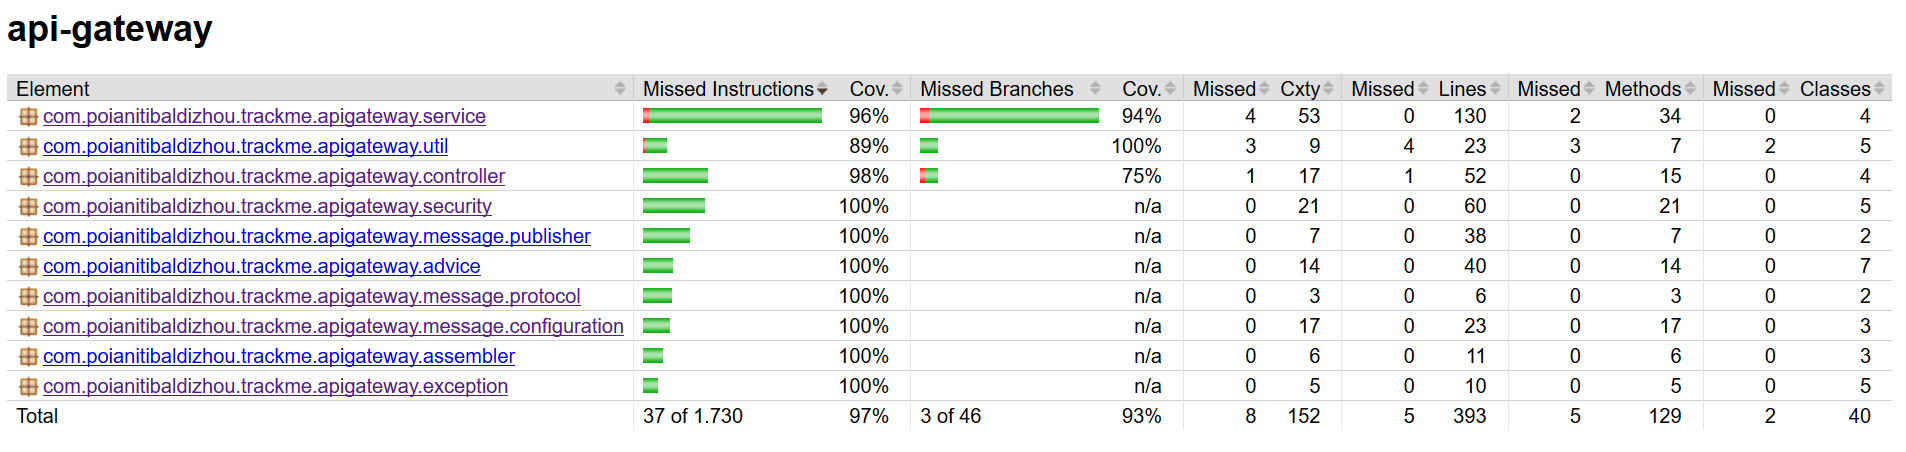
\includegraphics[width=\linewidth]{images/CoverageApigateway.png}
\caption{ API gateway coverage}
\label{fig:cvgapigateway}
\end{figure}


As one may notice, the entity and the filter packages are not present. Indeed, filters have been tested with JMeter, and therefore are not
present here. 
Furthermore, entity classes are basically only attributes and methods that are not shown since they are auto generated with lombok. \\
Finally, all the other lombok auto generated methods have been excluded from the coverage.

\par 
Similar reasoning applies also to the coverage of the individual request service.
\begin{figure}[H]
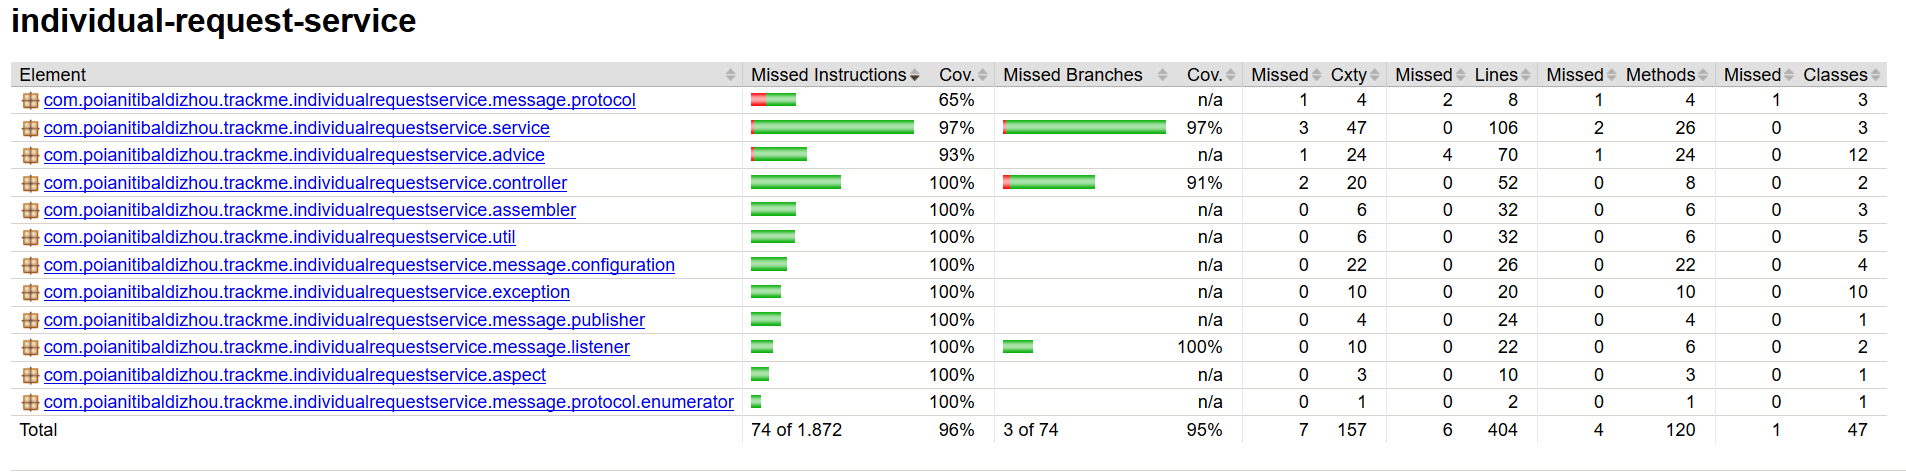
\includegraphics[width=\linewidth]{images/CoverageIndividualrequestservice.png}
\caption{ Individual request service coverage}
\label{fig:cvgindividual}
\end{figure}

\par 
Same things hold also for the group request service.
\begin{figure}[H]
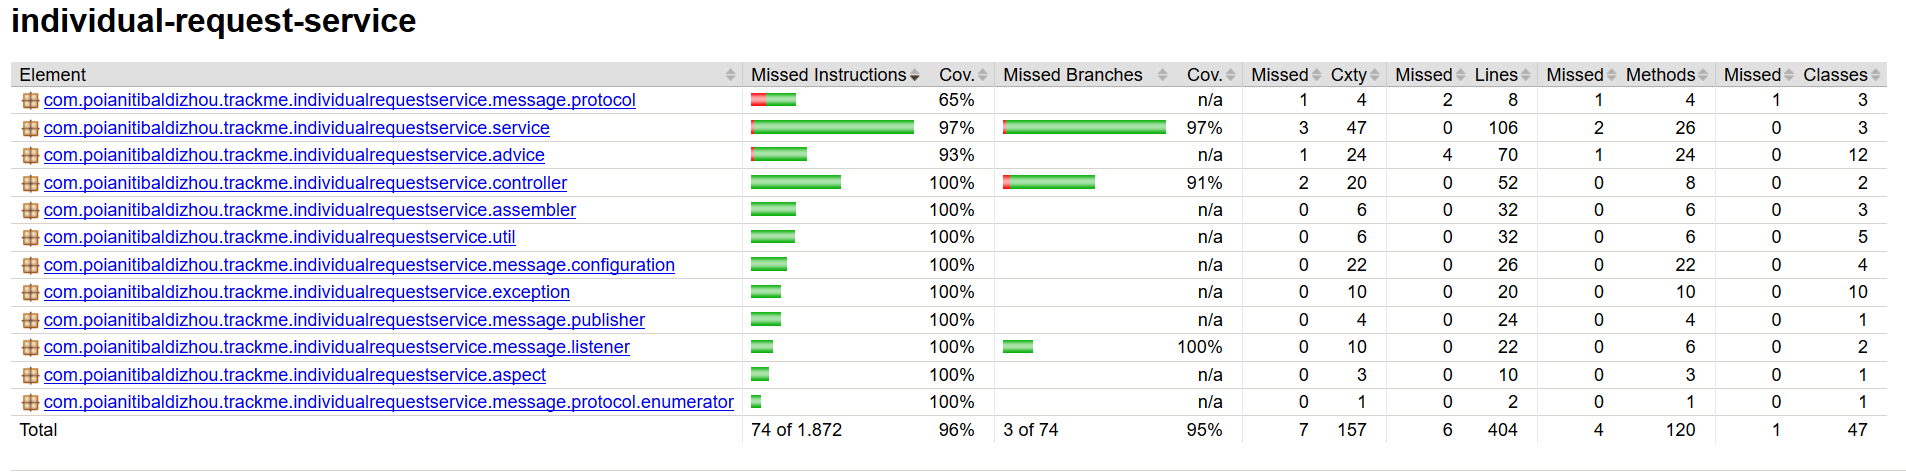
\includegraphics[width=\linewidth]{images/CoverageIndividualrequestservice.png}
\caption{ Group request individual service coverage}
\label{fig:cvggroup}
\end{figure}

\par
For what concerns the share data service, here follows the image of the coverage. The same comments
are valid also in this situation.

\begin{figure}[H]
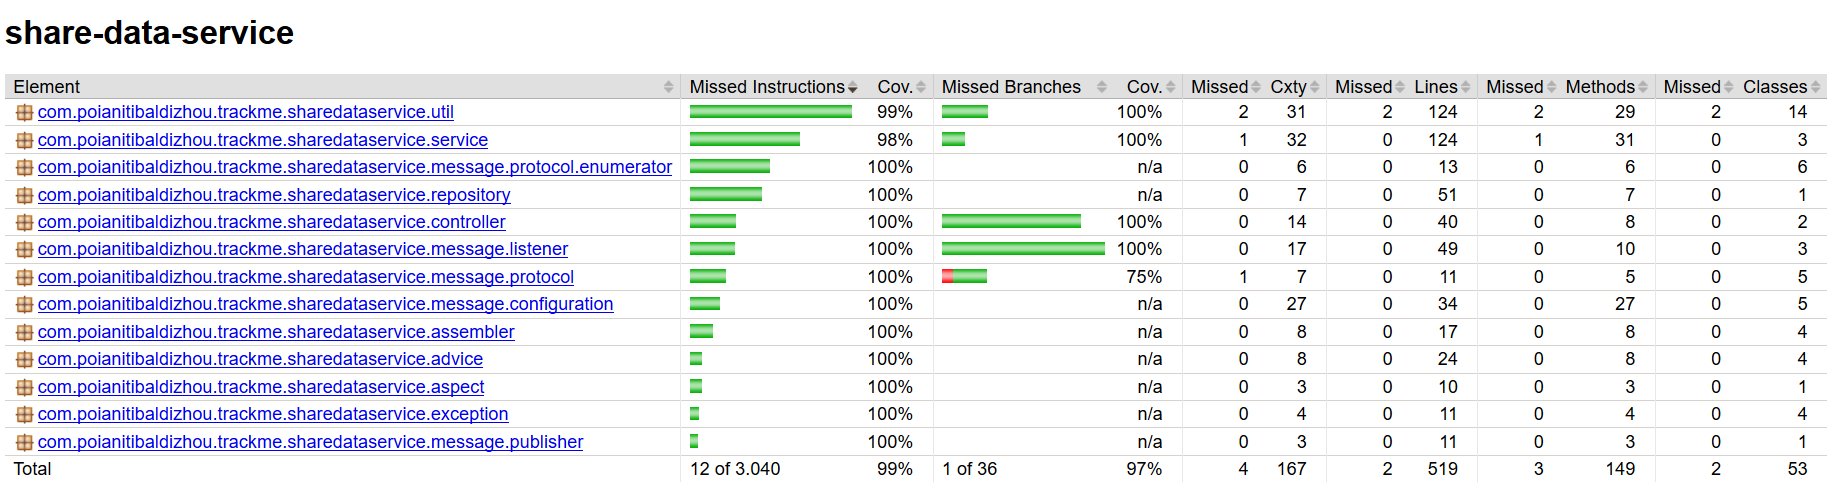
\includegraphics[width=\linewidth]{images/CoverageSharedataservice.png}
\caption{ Share data service coverage}
\label{fig:cvgshare}
\end{figure}


\subsubsection{JMeter} 
In order to do system testing on the server side of the project, JMeter has been adopted. There are many motivation for this choice: 
open-source application, user friendly (GUI), and many functionality such as the possibility of doing functional testing, load testing. Moreover it provides the possibility of testing almost every kind of resources: databases, message brokers, HTTP REST APIs and 
many other. In the end, to check if the system as a whole was working as expected, the following test plan has been written:
\begin{itemize}
\item Functional testing: without taking into consideration the concurrency and performance problems, the test plan focuses on 
the expected return value of each request, to test if the system works as intended. It has also been checked the group 
request accepted case when a group request is correlated to more than 1000 users. The test, basically, does not check the response body of each request, but it just checks the correct flow of the server application by making request in which the status code of each request is of type 20X.
\item Load testing: with the help of the "Random Controller", a random choice in the HTTP requests is applied and many thread 
users have been launched to test the maximum load of the system. In the GUI mode, the test results in a latency of more than 
20 seconds which the API Gateway discards due to a timeout. If the test has been done in a non-GUI mode, the average latency 
of a request would be less.
\item Real simulation testing: it is just a variation of the load testing with the ThinkTime added: a simulation of a possible think time 
of the user in order to make a request.
\end{itemize}
There are some considerations taken during the execution of the test plans:
\begin{itemize}
\item Since the server application is an eventually consistent system, then for example if a user register the api-gateway add immediately the user, but the other services will be consistent with this new information only when they will receive the message from the message broker (RabbitMQ) and after consumed it. Therefore some heuristics waiting time has been added on the test to wait for the eventually consistency of the system.
\item The test has been done locally with many applications opened, which could have interfered with the load testing.
\item The services has been deployed all on the same machine which was different from the deployment diagram.
\item Every time a test is launched, all the queues of the message broker are purged and the all tuples inside the DBs are deleted.
\item Remember that the server has a timeout of one minute for each request, after that the server will stop the request.
\item The time and date are not synchronized on a unique timezone or something like that with the clients (jmeter or app), due to complexity, therefore it is important to note that if the test is done within one hour before the midnight some tests could fail since the timestamp saved on the server could leap by one hour.
\end{itemize}


\subsection{Android application}
The test that has been done here are only about the health service which it is responsible to the Automated SOS service. This is the most important test since it could be a problem of life and death for the person using the application. Therefore, many test has been done:
\begin{itemize}
\item Unit tests of simple POJO classes that can be found in the folder app/src/test
\item Android tests, which are more complicated tests that need to be launched on real devices or emulators: from these test, there are unit tests, integrated tests and performance test. The last one it simply checks the average time to execute a call when a bluetooth message containing a grave health data is received. Other tests just checks the functionality of the classes with the exception of 
bluetooth which is really difficult to test since the emulator cannot simulate a bluetooth connection.
\\\\
\end{itemize}
